\documentclass[runningheads]{llncs}
\usepackage[T1]{fontenc}
\usepackage{lmodern}
\usepackage{amsmath,amssymb}
\usepackage{booktabs}
\usepackage{graphicx}
\usepackage{microtype}
\usepackage{xcolor}
\usepackage{algorithm}
\usepackage{algpseudocode}
\usepackage[colorlinks=true,linkcolor=blue!50!black,citecolor=blue!50!black,urlcolor=blue!50!black]{hyperref}

\newcommand{\E}{\mathbb{E}}
\newcommand{\conv}{\operatorname{conv}}
\newcommand{\TV}{\operatorname{TV}}
\newcommand{\AggAtsDelta}{-0.487}
\newcommand{\AggAtsEce}{0.078}
\newcommand{\AggAtsEceDown}{75}
\newcommand{\AggAtsHarm}{74}
\newcommand{\AggAtsHarmRate}{14.8}
\newcommand{\AggEvoDelta}{-0.473}
\newcommand{\AggEvoEce}{0.084}
\newcommand{\AggEvoEceDown}{87}
\newcommand{\AggEvoHarm}{8}
\newcommand{\AggEvoHarmRate}{1.6}
\newcommand{\AggMrtsDelta}{-0.368}
\newcommand{\AggMrtsEce}{0.131}
\newcommand{\AggMrtsEceDown}{77}
\newcommand{\AggMrtsHarm}{1}
\newcommand{\AggMrtsHarmRate}{0.2}
\newcommand{\AggPooledDelta}{-0.490}
\newcommand{\AggPooledEce}{0.078}
\newcommand{\AggPooledEceDown}{77}
\newcommand{\AggPooledHarm}{58}
\newcommand{\AggPooledHarmRate}{11.6}
\newcommand{\AggRbDelta}{-0.462}
\newcommand{\AggRbEce}{0.092}
\newcommand{\AggRbEceDown}{86}
\newcommand{\AggRbHarm}{7}
\newcommand{\AggRbHarmRate}{1.4}
\newcommand{\AggThermoDelta}{-0.493}
\newcommand{\AggThermoEce}{0.075}
\newcommand{\AggThermoEceDown}{77}
\newcommand{\AggThermoHarm}{49}
\newcommand{\AggThermoHarmRate}{9.8}
\newcommand{\AucBeats}{0.69}
\newcommand{\AucTemplate}{0.92}
\newcommand{\CfourAtsDelta}{-0.485}
\newcommand{\CfourAtsEce}{0.124}
\newcommand{\CfourAtsEceDown}{75}
\newcommand{\CfourAtsHarm}{14}
\newcommand{\CfourEvoDelta}{-0.442}
\newcommand{\CfourEvoEce}{0.132}
\newcommand{\CfourEvoEceDown}{81}
\newcommand{\CfourEvoHarm}{7}
\newcommand{\CfourMrtsDelta}{-0.355}
\newcommand{\CfourMrtsEce}{0.160}
\newcommand{\CfourMrtsEceDown}{69}
\newcommand{\CfourMrtsHarm}{1}
\newcommand{\CfourPooledDelta}{-0.488}
\newcommand{\CfourPooledEce}{0.127}
\newcommand{\CfourPooledEceDown}{76}
\newcommand{\CfourPooledHarm}{13}
\newcommand{\CfourRbDelta}{-0.437}
\newcommand{\CfourRbEce}{0.134}
\newcommand{\CfourRbEceDown}{85}
\newcommand{\CfourRbHarm}{7}
\newcommand{\CfourTempIdEce}{0.068}
\newcommand{\CfourTempPooledHarm}{6}
\newcommand{\CfourThermoDelta}{-0.490}
\newcommand{\CfourThermoEce}{0.124}
\newcommand{\CfourThermoEceDown}{78}
\newcommand{\CfourThermoHarm}{13}
\newcommand{\ConeAtsDelta}{-0.263}
\newcommand{\ConeAtsEce}{0.056}
\newcommand{\ConeAtsEceDown}{18}
\newcommand{\ConeAtsHarm}{7}
\newcommand{\ConeEvoDelta}{-0.266}
\newcommand{\ConeEvoEce}{0.055}
\newcommand{\ConeEvoEceDown}{26}
\newcommand{\ConeEvoHarm}{0}
\newcommand{\ConeMrtsDelta}{-0.201}
\newcommand{\ConeMrtsEce}{0.090}
\newcommand{\ConeMrtsEceDown}{24}
\newcommand{\ConeMrtsHarm}{0}
\newcommand{\ConePooledDelta}{-0.257}
\newcommand{\ConePooledEce}{0.064}
\newcommand{\ConePooledEceDown}{20}
\newcommand{\ConePooledHarm}{7}
\newcommand{\ConeRbDelta}{-0.256}
\newcommand{\ConeRbEce}{0.062}
\newcommand{\ConeRbEceDown}{26}
\newcommand{\ConeRbHarm}{0}
\newcommand{\ConeThermoDelta}{-0.262}
\newcommand{\ConeThermoEce}{0.059}
\newcommand{\ConeThermoEceDown}{19}
\newcommand{\ConeThermoHarm}{5}
\newcommand{\CthreeAtsDelta}{-0.304}
\newcommand{\CthreeAtsEce}{0.052}
\newcommand{\CthreeAtsEceDown}{43}
\newcommand{\CthreeAtsHarm}{9}
\newcommand{\CthreeEvoDelta}{-0.290}
\newcommand{\CthreeEvoEce}{0.057}
\newcommand{\CthreeEvoEceDown}{51}
\newcommand{\CthreeEvoHarm}{0}
\newcommand{\CthreeMrtsDelta}{-0.232}
\newcommand{\CthreeMrtsEce}{0.083}
\newcommand{\CthreeMrtsEceDown}{46}
\newcommand{\CthreeMrtsHarm}{0}
\newcommand{\CthreePooledDelta}{-0.305}
\newcommand{\CthreePooledEce}{0.051}
\newcommand{\CthreePooledEceDown}{45}
\newcommand{\CthreePooledHarm}{7}
\newcommand{\CthreeRbDelta}{-0.285}
\newcommand{\CthreeRbEce}{0.061}
\newcommand{\CthreeRbEceDown}{47}
\newcommand{\CthreeRbHarm}{0}
\newcommand{\CthreeThermoDelta}{-0.306}
\newcommand{\CthreeThermoEce}{0.049}
\newcommand{\CthreeThermoEceDown}{45}
\newcommand{\CthreeThermoHarm}{5}
\newcommand{\CtwoAtsDelta}{-0.315}
\newcommand{\CtwoAtsEce}{0.072}
\newcommand{\CtwoAtsEceDown}{38}
\newcommand{\CtwoAtsHarm}{12}
\newcommand{\CtwoEvoDelta}{-0.321}
\newcommand{\CtwoEvoEce}{0.063}
\newcommand{\CtwoEvoEceDown}{50}
\newcommand{\CtwoEvoHarm}{0}
\newcommand{\CtwoMrtsDelta}{-0.265}
\newcommand{\CtwoMrtsEce}{0.088}
\newcommand{\CtwoMrtsEceDown}{47}
\newcommand{\CtwoMrtsHarm}{0}
\newcommand{\CtwoPooledDelta}{-0.319}
\newcommand{\CtwoPooledEce}{0.071}
\newcommand{\CtwoPooledEceDown}{38}
\newcommand{\CtwoPooledHarm}{9}
\newcommand{\CtwoRbDelta}{-0.316}
\newcommand{\CtwoRbEce}{0.066}
\newcommand{\CtwoRbEceDown}{50}
\newcommand{\CtwoRbHarm}{0}
\newcommand{\CtwoThermoDelta}{-0.323}
\newcommand{\CtwoThermoEce}{0.067}
\newcommand{\CtwoThermoEceDown}{38}
\newcommand{\CtwoThermoHarm}{7}
\newcommand{\FrontBetter}{0}
\newcommand{\FrontEvals}{16796}
\newcommand{\FrontMaxPts}{646}
\newcommand{\FrontMaxWorse}{1.3e-03}
\newcommand{\FrontMinPts}{7}
\newcommand{\FrontPairs}{68}
\newcommand{\FrontWorse}{3}
\newcommand{\HarmRatio}{6}
\newcommand{\LotoAtsDelta}{-0.600}
\newcommand{\LotoAtsEce}{0.069}
\newcommand{\LotoAtsEceDown}{199}
\newcommand{\LotoAtsHarm}{32}
\newcommand{\LotoAvgIdHarm}{0}
\newcommand{\LotoAvgIdRaw}{-0.290}
\newcommand{\LotoAvgIdSame}{+0.000}
\newcommand{\LotoAvgPeerRaw}{-0.605}
\newcommand{\LotoAvgPeerSame}{-0.315}
\newcommand{\LotoAvgPooledHarm}{22}
\newcommand{\LotoAvgPooledRaw}{-0.652}
\newcommand{\LotoAvgPooledSame}{-0.362}
\newcommand{\LotoAvgRbRaw}{-0.587}
\newcommand{\LotoAvgRbSame}{-0.298}
\newcommand{\LotoAvgThermoHarm}{17}
\newcommand{\LotoAvgThermoRaw}{-0.654}
\newcommand{\LotoAvgThermoSame}{-0.364}
\newcommand{\LotoEvoDelta}{-0.591}
\newcommand{\LotoEvoEce}{0.081}
\newcommand{\LotoEvoEceDown}{225}
\newcommand{\LotoEvoHarm}{1}
\newcommand{\LotoMrtsDelta}{-0.451}
\newcommand{\LotoMrtsEce}{0.146}
\newcommand{\LotoMrtsEceDown}{197}
\newcommand{\LotoMrtsHarm}{0}
\newcommand{\LotoPeerDelta}{-0.583}
\newcommand{\LotoPeerHarm}{1}
\newcommand{\LotoPooledDelta}{-0.605}
\newcommand{\LotoPooledEce}{0.068}
\newcommand{\LotoPooledEceDown}{204}
\newcommand{\LotoPooledHarm}{22}
\newcommand{\LotoRbDelta}{-0.573}
\newcommand{\LotoRbEce}{0.092}
\newcommand{\LotoRbEceDown}{224}
\newcommand{\LotoRbHarm}{0}
\newcommand{\LotoRelaxDelta}{-0.556}
\newcommand{\LotoRelaxHarm}{7}
\newcommand{\LotoThermoDelta}{-0.607}
\newcommand{\LotoThermoEce}{0.065}
\newcommand{\LotoThermoEceDown}{204}
\newcommand{\LotoThermoHarm}{19}
\newcommand{\NCfour}{100}
\newcommand{\NCone}{30}
\newcommand{\NCthree}{60}
\newcommand{\NCtwo}{60}
\newcommand{\NLoto}{250}
\newcommand{\NTotal}{500}
\newcommand{\OracleDelta}{-0.613}
\newcommand{\RetainEvo}{96}
\newcommand{\SwitchCfourDelta}{-0.447}
\newcommand{\SwitchCfourHarm}{10}
\newcommand{\SwitchLotoDelta}{-0.607}
\newcommand{\SwitchLotoHarm}{2}
\newcommand{\TaxEvo}{4}

\makeatletter
\newcommand{\inputtable}[1]{\@@input #1 }
\makeatother

\begin{document}
\title{The Confidence Tax: Evolving Regret-Budgeted Temperature Fields for Safe Calibration Transfer in Language Models}
\titlerunning{The Confidence Tax}
\author{Anonymous Authors}
\authorrunning{Anonymous Authors}
\institute{Anonymous Institution}
\maketitle

\begin{abstract}
A calibrator for the answer probabilities of a language model is usually fitted on labelled source tasks and then applied to new, unlabelled tasks.
Fitting the pooled log-loss improves the average but makes a sizeable fraction of new tasks worse; requiring that no source gets worse often leaves the model unchanged.
We cast calibration transfer as a many-objective problem with one regret objective per source task and solve its $\varepsilon$-constraint scalarisation: minimise the pooled log-loss subject to a budget on a confidence bound of every source's regret, over a label-free temperature field that also reads answer-order consistency.
Evolution strategies enter in two ways.
CMA-ES maps the empirical Pareto front between mean gain and worst-source regret and certifies that the gradient-based solutions of the non-convex constrained problem are not improved by a global search (0 of \FrontPairs{} problems).
A bilevel variant, Evo-RB, evolves the structure of the field (radial-basis centres and bandwidth) with CMA-ES while the weights are solved exactly under the budget.
On five open-weight models, two prompts and \NTotal{} target task units from five evaluation rosters, four of them sealed and pre-registered, Evo-RB harms \AggEvoHarm{} units (\AggEvoHarmRate\%), against \AggThermoHarm--\AggAtsHarm{} (\AggThermoHarmRate--\AggAtsHarmRate\%) for pooled temperature scaling, Thermometer and adaptive temperature scaling, lowers expected calibration error on \AggEvoEceDown\% and the Brier score on \AggEvoBrierDown\% of units against \AggThermoEceDown\% and \AggThermoBrierDown\%, and retains \RetainEvo\% of their mean log-loss gain: a confidence tax of about \TaxEvo\% of the gain buys roughly \HarmRatio{} times fewer harmed tasks.
\keywords{Calibration \and Evolution strategies \and Multi-objective optimisation \and Language models \and Transfer learning}
\end{abstract}

\section{Introduction}
Language models that answer multiple-choice questions produce a distribution over the options, and this distribution is often miscalibrated: the confidence of the top answer does not match its accuracy~\cite{kadavath2022know,zhao2021calibrate}.
Temperature scaling~\cite{guo2017calibration} repairs this with one parameter fitted on labelled data from the task at hand.
A deployed model, however, meets tasks without labels, so the calibrator has to be learned on labelled \emph{source} tasks and transferred~\cite{yu2022multidomain,shen2024thermometer,xie2024ats}.

Transfer raises a question that averages hide: \emph{how many tasks does the calibrator make worse?}
A calibrator that fits the pooled log-loss of many sources moves where most sources benefit.
The tasks on which the model is already calibrated pay for it.
In our data pooled temperature scaling, a probability-feature adaptation of Thermometer~\cite{shen2024thermometer} and one of adaptive temperature scaling (ATS)~\cite{xie2024ats} each increase the log-loss by more than 0.01 nats on 10--15\% of target task units (Table~\ref{tab:main}).
The opposite design, minimax-regret temperature scaling~\cite{calport2026}, never makes a source worse, but whenever one source is over- and another underconfident it provably returns the identity and does nothing.

We treat the per-source regrets as what they are: \emph{objectives}.
With $W$ source tasks, a calibrator induces a vector of $W$ regrets, and pooled fitting, minimax fitting and our proposal are three scalarisations of the same many-objective problem (weighted sum, Chebyshev, and $\varepsilon$-constraint~\cite{miettinen1999nonlinear}).
The $\varepsilon$-constraint form fits the deployment goal directly: maximise the average gain while every source's regret stays below a small budget.
The part of the average gain that a safe calibrator gives up relative to an unconstrained one is what we call the \emph{confidence tax}; the question is how small the tax can be made for a given level of protection.
We place the budget on a case-clustered upper confidence bound, which makes the problem non-convex, and we use a label-free temperature field whose inputs include how much the model changes its answer when the options are reordered.

The contributions are:
\begin{itemize}
\item \textbf{Regret-budgeted calibration (RB-Cal)} as the $\varepsilon$-constraint scalarisation of the per-source regret objectives, with a statistical budget, a source-only model selection rule and a significance-based deployment gate (Section~\ref{sec:method}).
\item \textbf{An evolutionary analysis and extension.} CMA-ES~\cite{hansen2001cma} maps the Pareto front of mean gain against worst-source regret and certifies the gradient-based solutions of the non-convex problem; \textbf{Evo-RB} evolves the structure of the temperature field with CMA-ES in a bilevel loop and improves on the fixed structure on every roster (Section~\ref{sec:evo}).
\item \textbf{A sequence of sealed, pre-registered evaluations}: four rosters of unseen tasks, each opened once after the method under test was frozen, plus leave-one-task-out over 25 sources; \NTotal{} target task units in all, with harm counts reported for every method, including a roster on which our method harms seven units (Section~\ref{sec:results}).
\end{itemize}

\section{Related Work}
\paragraph{Calibration transfer.}
Temperature scaling and its richer variants~\cite{guo2017calibration,balanya2024adaptive,rahimi2020intra,zhang2020mixnmatch,lecoz2024tva} assume labels from the deployment distribution.
Multi-domain temperature scaling~\cite{yu2022multidomain}, domain-generalisation calibration~\cite{gong2021dgcal,choi2024cts} and TransCal~\cite{wang2020transcal} learn from several labelled domains.
For language models, Thermometer~\cite{shen2024thermometer} predicts a task temperature from unlabelled inputs and ATS~\cite{xie2024ats} a per-token temperature from hidden states.
All of them optimise an average over sources.
Minimax-regret temperature scaling~\cite{calport2026} bounds every source but is inert under conflicting sources; hidden miscalibration regimes are mapped in~\cite{kobalczyk2026hidden}.
\paragraph{Constrained and robust learning.}
Group DRO~\cite{sagawa2020dro} minimises the worst group loss and PAC constrained learning~\cite{chamon2020pac} an average under constraints; confidence-bound constraints follow high-confidence policy improvement and Seldonian algorithms~\cite{thomas2015hcpi,thomas2019seldonian}, and Learn-then-Test~\cite{angelopoulos2021ltt} gives finite-sample risk control.
The common-descent geometry we use for diagnosis is that of MGDA~\cite{desideri2012mgda,sener2018mtl,liu2021cagrad}.
\paragraph{Evolutionary computation for learning.}
CMA-ES~\cite{hansen2001cma,hansen2016tutorial} is a standard derivative-free optimiser for continuous, non-convex problems and is used for hyperparameter optimisation~\cite{loshchilov2016cmahpo}; evolutionary search over model structure is established in architecture search~\cite{real2019regularized}; multi-objective evolutionary algorithms such as NSGA-II~\cite{deb2002nsga2} approximate Pareto fronts, and constraint handling by penalties and repair is surveyed in~\cite{coello2002constraint}.
To our knowledge, evolutionary search has not been used to map or solve the per-source trade-off of calibration transfer.

\section{Problem}\label{sec:problem}
A \emph{unit} is a model--prompt pair with its own calibrator.
For a question with $K$ options the unit returns $p\in\Delta^{K-1}$ (floored at $10^{-12}$ and renormalised); a calibrator returns $q_\theta(\cdot\mid p)$ and the identity $\theta_0$ returns $p$.
Source task $w\in\{1,\dots,W\}$ has distribution $D_w$ over $(p,y)$, and the \emph{regret} of $\theta$ on $w$ is
\begin{equation}
\Delta_w(\theta)=\E_{D_w}\big[-\log q_\theta(y\mid p)+\log p_y\big],\qquad\Delta_w(\theta_0)=0.
\end{equation}
Negative regret is improvement.
A target task unit is \emph{harmed} when its regret exceeds 0.01 nats.
The vector $(\Delta_1,\dots,\Delta_W)$ defines a $W$-objective problem.
Pooled fitting minimises $\sum_w\pi_w\Delta_w$ with $\pi_w=n_w/n$; minimax fitting minimises $\max_w\Delta_w$; both are points of the Pareto set, and neither controls the trade-off between them.

For calibrators whose logits are linear in $\theta$ every $\Delta_w$ is convex, and the identity is the minimax solution if and only if $0\in\conv\{\nabla\Delta_w(\theta_0)\}_w$ (the max rule for subdifferentials).
For the scalar temperature $q\propto p^\beta$, $\nabla\Delta_w(\theta_0)=\E_{D_w}[-\log p_y]-\E_{D_w}[H(p)]$, so one overconfident source (log-loss above mean entropy) and one underconfident source pin the minimax solution to the identity~\cite{calport2026}.
With 25 heterogeneous sources this happens for three of our ten units.
Conversely, any budget $\varepsilon>0$ leaves the identity whenever the pooled loss has a descent direction, because the constraints are slack at $\theta_0$.

\section{Method}\label{sec:method}
\paragraph{Temperature field.}
RB-Cal tempers the probabilities, $q_k\propto p_k^{\beta(x)}$, with an inverse temperature that depends on label-free features of the input:
\begin{equation}
\beta(x)=b_0+v^\top\psi(z(x)),\qquad \psi_j(z)=J^{-1/2}\exp\!\big(-\|z-c_j\|^2/2\sigma^2\big),
\end{equation}
with $\|v\|_2\le\min(b_0-0.25,\,4-b_0)$, which keeps $\beta\in[0.25,4]$ for every input because $\|\psi\|\le1$.
The feature vector $z$ has five entries: normalised entropy, top-1 probability and the gap between the two largest probabilities; the total variation between the option distributions the model gives under two answer orders (mapped back to the same options); and the mean of that quantity over the unlabelled batch of the same task.
Order sensitivity marks unreliable confidence~\cite{pezeshkpour2024order,zheng2024pride}: on our source data, rows whose answer does not change under reordering are close to calibrated on easy tasks, and rows that change are strongly overconfident.
Answer orders are part of the standard scoring of multiple-choice items; the feature needs two forward passes per question and no labels.
The centres $c_j$ are chosen on source inputs by farthest-point traversal, and the logits are linear in $\theta=(b_0,v)$.

\paragraph{Regret budget.}
With empirical regrets $\hat\Delta_w$ on the training cases of source $w$ and their standard errors $\widehat{\mathrm{SE}}_w$ clustered by question,
\begin{equation}\label{eq:rbcal}
\min_\theta\ \sum_w\pi_w\hat\Delta_w(\theta)+\lambda\|v\|_2^2\quad\text{s.t.}\quad\hat\Delta_w(\theta)+z\,\widehat{\mathrm{SE}}_w(\theta)\le\varepsilon\ \ \forall w,
\end{equation}
with $\varepsilon=0.01$ (the harm threshold) and $z=1.645$.
The margin keeps noisy sources from using the whole budget; it also makes the feasible set non-convex.
The default solver is SLSQP from the identity with analytic gradients; a solution is accepted only if every constraint holds to $10^{-7}$.

\paragraph{Selection and gate.}
$J\in\{0,1,2,4,8\}$, $\sigma\in\{0.2,0.5,1\}$ and $\lambda\in\{0,0.01,0.1\}$ give 37 configurations, chosen by leave-one-source-out on the training split (fewest held-out sources above $\varepsilon$, then mean held-out regret, then simplicity).
The refitted calibrator is deployed unless some source shows a significant violation on a disjoint selection split, $\hat\Delta^{\mathrm{sel}}_w-1.645\,\widehat{\mathrm{SE}}^{\mathrm{sel}}_w>\varepsilon$; otherwise the identity is deployed.
No step reads target labels.

\paragraph{Transfer.}
If the log-ratio $-\log q_\theta(y\mid p)+\log p_y$ is bounded by $B$, then for any target $D_T$ and weights $\mu\in\Delta^{W-1}$, $\Delta_T(\theta)\le\sum_w\mu_w\Delta_w(\theta)+2B\,\TV(D_T,\sum_w\mu_wD_w)$, because the regret is linear in the distribution.
A per-source budget therefore controls every target close to a mixture of sources, which an average budget does not; targets far from all mixtures are not controlled, and Section~\ref{sec:results} shows a roster where this matters.

\section{Evolutionary Components}\label{sec:evo}
\paragraph{CMA-ES on the constrained problem.}
We solve~\eqref{eq:rbcal} with CMA-ES~\cite{hansen2001cma} (pycma, population of default size, $\sigma_0=0.1$, 3000 evaluations, seed 1).
The bounds on $\beta$ are kept by a repair operator that projects every candidate onto the admissible field, the budget by a penalty of 100 per nat of violation~\cite{coello2002constraint}, and an elitist archive keeps the best feasible candidate ever evaluated; the identity is always feasible, so the solver never returns an infeasible field.
Running it for budgets $\varepsilon\in\{0,0.0025,0.005,0.01,0.02,0.05,0.1\}$ and logging every evaluated candidate as a point (pooled regret, worst-source bound) yields an empirical Pareto front of the two quantities the deployment trades off.

\paragraph{Evo-RB: evolving the structure of the field.}
The farthest-point centres and the bandwidth menu are a fixed, hand-designed structure.
Evo-RB optimises them in a bilevel loop.
The outer level is CMA-ES over the $J\times5$ centre coordinates and $\log\sigma$ (300 evaluations, $\sigma_0=0.05$, started at the farthest-point centres; $J$ and $\lambda$ are those chosen by leave-one-source-out).
For each candidate structure the inner level solves~\eqref{eq:rbcal} exactly for $\theta$ on the training split.
The fitness is the mean regret on the selection split plus a penalty of 100 per unit of significant budget violation there.
Because the selection split is now used for fitness, the deployment gate moves to the third, untouched audit split.
Constant-temperature units (no structure) are left unchanged.
On one CPU thread and one unit (14{,}744 training rows), fitting Evo-RB takes \TimeEvo{}\,s, against \TimeRbFit{}\,s for one RB-Cal fit and \TimePooled{}\,s for pooled TS; the leave-one-source-out choice of $(J,\lambda)$, shared by both, takes about \TimeLosoMin{}\,min, and applying any calibrator to 3000 target rows takes under 0.2\,s.
All of this is offline and per model--prompt pair; RB-Cal and Evo-RB additionally need both answer orders at prediction time, which doubles the language-model inference.
Algorithm~\ref{alg:evorb} summarises the procedure.

\begin{algorithm}[t]
\caption{Evo-RB for one unit (model--prompt pair).}\label{alg:evorb}
\begin{algorithmic}[1]
\Require source splits \textit{train}, \textit{select}, \textit{audit}; $J,\lambda$ from leave-one-source-out; $\varepsilon=0.01$, $z=1.645$
\State $C\gets$ $J$ farthest-point centres of the features of \textit{train};\ $s\gets\log\sigma$
\State start CMA-ES at $(C,s)$ with step size $0.05$
\While{fewer than 300 candidates evaluated}
  \For{each candidate $(C',s')$ of the population}
    \State $\theta^\ast\gets$ solution of~\eqref{eq:rbcal} on \textit{train} with centres $C'$, bandwidth $e^{s'}$ \Comment{inner, exact}
    \State $f\gets\overline{\Delta}^{\textit{select}}(\theta^\ast)+100\sum_w\max\{0,\ \hat\Delta^{\textit{select}}_w-1.645\,\widehat{\mathrm{SE}}^{\textit{select}}_w-\varepsilon\}$
  \EndFor
  \State update the CMA-ES distribution with the fitnesses; keep the best candidate and its $\theta^\ast$
\EndWhile
\State \Return $\theta^\ast$ if no source has $\hat\Delta^{\textit{audit}}_w-1.645\,\widehat{\mathrm{SE}}^{\textit{audit}}_w>\varepsilon$, else the identity
\end{algorithmic}
\end{algorithm}

\section{Experimental Protocol}\label{sec:protocol}
\paragraph{Models and probabilities.}
Qwen3.5-9B, Gemma-4-12B-it, Granite-4.2-8B, Ministral-3-8B-Instruct-2512 and Olmo-3-7B-Instruct, at fixed repository commits, in bf16 with their chat templates and two prompts that end with an assistant prefix (\texttt{Answer:} and \texttt{The answer is (}).
The option probability is the next-token probability of the option letter, renormalised over the options.
Every question is scored under two answer orders; all rows of a question form one case.
This gives ten units.
Sources and C1 were scored on one software stack and C2--C4 on a later one (same model commits and code, newer PyTorch); re-scoring 372 source rows per model on the later stack changes the mean log-loss by at most 0.008 nats for four models and by 0.026 for Gemma-4-12B, which is slightly sharper.
All methods see the same target probabilities, so comparisons within a roster are paired.

\paragraph{Sources and rosters.}
The 25 sources are ARC-Easy/Challenge~\cite{clark2018arc}, BoolQ~\cite{clark2019boolq}, HellaSwag~\cite{zellers2019hellaswag}, LogiQA~\cite{liu2020logiqa}, four MMLU groups~\cite{hendrycks2021mmlu}, 14 MMLU-Pro categories~\cite{wang2024mmlupro}, OpenBookQA~\cite{mihaylov2018obqa} and WinoGrande~\cite{sakaguchi2020winogrande} (at most 500 questions each; cases split 60/20/20 into training, selection and audit).
Targets are never used for fitting or selection.
\textbf{C1}: AQuA-RAT~\cite{ling2017aqua}, PIQA~\cite{bisk2020piqa}, SciQ~\cite{welbl2017sciq}.
\textbf{C2}: QASC~\cite{khot2020qasc}, RACE-high~\cite{lai2017race}, Social IQa~\cite{sap2019socialiqa}, Cosmos QA~\cite{huang2019cosmos}, MedQA~\cite{jin2021medqa}, Belebele (English)~\cite{bandarkar2024belebele}.
\textbf{C3}: QuaRTz~\cite{tafjord2019quartz}, ScienceQA (text)~\cite{lu2022scienceqa}, PubMedQA~\cite{jin2019pubmedqa}, Balanced COPA~\cite{kavumba2019copa}, LSAT-LR and LSAT-RC from AGIEval~\cite{zhong2024agieval}.
\textbf{C4}: nine BIG-bench tasks~\cite{srivastava2023bigbench} (date understanding, disambiguation, logical deduction, temporal sequences, StrategyQA, implicatures, tracking shuffled objects, epistemic reasoning, navigate) and SAT-English from AGIEval.
\textbf{LOTO}: each source task held out in turn, all methods refitted on the other 24, all rows of the held-out task scored (250 units).
Each roster was built after the method it tested had been frozen and pre-registered with its endpoints, and was scored once: C1 tested the first RB-Cal version (scalar features), C2 a revised gate, C3 the order-consistency field reported here as RB-Cal, and C4 a task-level switching rule that failed (Section~\ref{sec:negative}).
RB-Cal was therefore frozen before C3 and C4 existed; C1 and C2 are secondary for it.
Evo-RB was designed after all rosters had been opened; its acceptance rule (at most one more harmed LOTO unit than RB-Cal and a mean gain at least 0.005 nats larger) was written down before it was run, and its roster results are secondary.
The LOTO runs reuse the field configuration selected on all 25 sources.

\paragraph{Baselines.}
Pooled temperature scaling (pooled TS) and minimax-regret TS (MRTS)~\cite{calport2026}, both on a 241-point logarithmic grid in $[0.25,4]$.
Thermometer-P and ATS-P adapt Thermometer~\cite{shen2024thermometer} and ATS~\cite{xie2024ats} to the same probability features (8 centres, $\sigma=0.5$, $L_2$ penalty $10^{-3}$, fixed in advance): Thermometer-P averages per-input temperatures over the unlabelled task batch and weights source tasks equally; ATS-P predicts a per-input inverse temperature and uses the selective-smoothing loss with $\alpha=0.5$.
They are adaptations, not reproductions: the originals read hidden states.

\paragraph{Metrics.}
Per target task unit (model $\times$ prompt $\times$ task) we report the change in log-loss relative to the uncalibrated model ($\Delta$, lower is better), harm ($\Delta>0.01$), ECE with 15 equal-width bins on the top-1 confidence, and the Brier score
\begin{equation}
\mathrm{BS}=\sum_{k=1}^{K}\big(q_k-\mathbf{1}[y=k]\big)^2,
\end{equation}
a second strictly proper scoring rule, averaged over the rows of the unit; $q$ is the calibrated distribution ($q=p$ for the uncalibrated model), and the sum runs over the $K$ options without division by $K$.
For ECE and Brier score we also report whether they decreased relative to the uncalibrated model.

\section{Results}\label{sec:results}
\begin{table}[t]
\centering
\caption{Mean $\Delta$NLL (nats; lower is better) and number of harmed task units (\#h, $\Delta>0.01$) on each roster, and the aggregate over all \NTotal{} units: harmed units, mean $\Delta$, mean Brier score (uncalibrated: \AggIdBrier), mean ECE, and the shares of units whose Brier score and ECE decreased ($\downarrow$). C1/C2/C3/C4: \NCone/\NCtwo/\NCthree/\NCfour{} units; LOTO: \NLoto{} units.}
\label{tab:main}
\setlength{\tabcolsep}{3.2pt}
\resizebox{\linewidth}{!}{%
\begin{tabular}{lcccccccccccccccc}
\toprule
& \multicolumn{2}{c}{C1} & \multicolumn{2}{c}{C2} & \multicolumn{2}{c}{C3} & \multicolumn{2}{c}{C4} & \multicolumn{2}{c}{LOTO} & \multicolumn{6}{c}{All \NTotal{} units}\\
\cmidrule(lr){2-3}\cmidrule(lr){4-5}\cmidrule(lr){6-7}\cmidrule(lr){8-9}\cmidrule(lr){10-11}\cmidrule(lr){12-17}
Method & $\Delta$ & \#h & $\Delta$ & \#h & $\Delta$ & \#h & $\Delta$ & \#h & $\Delta$ & \#h & \#h & $\Delta$ & Brier & Brier$\downarrow$ & ECE & ECE$\downarrow$\\
\midrule
\inputtable{generated/tab_main.tex}
\bottomrule
\end{tabular}}
\end{table}

\paragraph{Gain against harm.}
Table~\ref{tab:main} and Fig.~\ref{fig:frontier} give every method on every roster.
Pooled TS, Thermometer-P and ATS-P obtain the largest mean gains and harm \AggPooledHarm, \AggThermoHarm{} and \AggAtsHarm{} of \NTotal{} units.
MRTS harms one unit and gives up a quarter of the gain.
RB-Cal harms \AggRbHarm{} units and Evo-RB \AggEvoHarm, about \HarmRatio{} times fewer than the best unconstrained method, while Evo-RB keeps \RetainEvo\% of its mean gain (\AggEvoDelta{} against \AggThermoDelta).
On the two rosters on which RB-Cal was tested sealed (C3, C4) it harms \CthreeRbHarm{} and \CfourRbHarm{} units against \CthreeThermoHarm{} and \CfourThermoHarm{} for Thermometer-P.
On C1 and C2, Evo-RB matches or exceeds pooled TS in mean log-loss (\ConeEvoDelta{} vs.\ \ConePooledDelta; \CtwoEvoDelta{} vs.\ \CtwoPooledDelta) without harming any unit; these rosters are secondary for it.
No method dominates Evo-RB on both axes on any roster.

\begin{figure}[t]
\centering
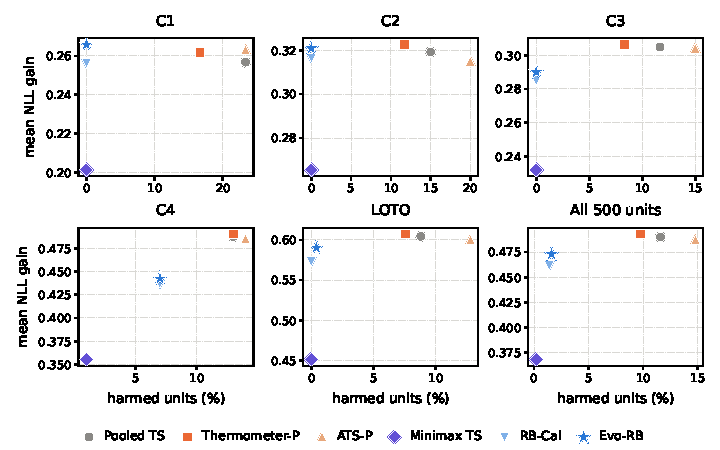
\includegraphics[width=\linewidth]{figures/frontier.pdf}
\caption{Mean log-loss gain against the share of harmed task units, per roster and over all \NTotal{} units. Up and to the left is better.}
\label{fig:frontier}
\end{figure}

\paragraph{Calibration error per unit.}
Fig.~\ref{fig:ece} plots the calibrated against the uncalibrated ECE of every held-out LOTO unit for Thermometer-P and Evo-RB.
Thermometer-P maps most units to a nearly constant ECE of about 0.05--0.1, a flat cloud; this is good for strongly miscalibrated units and bad for units that were already calibrated, which it pushes above the diagonal (orange crosses mark log-loss harm).
Evo-RB corrects strongly miscalibrated units less (its mean ECE is \AggEvoEce{} against \AggThermoEce{} over all units) but almost never moves a unit above the diagonal; it lowers ECE on \AggEvoEceDown\% of all units against \AggThermoEceDown\% for Thermometer-P, and on more units than every baseline on every roster.
The Brier score tells the same story.
The unconstrained methods have the lowest mean (\AggThermoBrier--\AggAtsBrier{} against \AggEvoBrier{} for Evo-RB and \AggIdBrier{} uncalibrated), a difference of half a hundredth, but Evo-RB lowers the Brier score on \AggEvoBrierDown\% of units, against \AggThermoBrierDown\% for Thermometer-P, \AggPooledBrierDown\% for pooled TS and \AggAtsBrierDown\% for ATS-P, again more units than every baseline on every roster.

\begin{figure}[t]
\centering
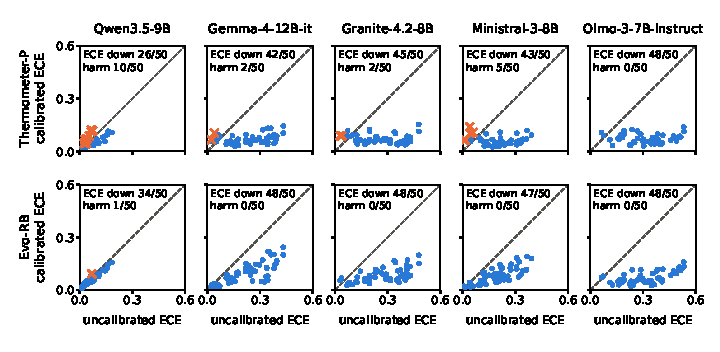
\includegraphics[width=\linewidth]{figures/ece_pair_loto.pdf}
\caption{Calibrated vs.\ uncalibrated ECE for the 250 held-out LOTO units (25 tasks $\times$ 2 prompts per model). Below the diagonal is lower ECE; crosses are units whose log-loss got worse by more than 0.01 nats.}
\label{fig:ece}
\end{figure}

\paragraph{What the evolution strategy finds.}
On the ten development units and seven budgets, CMA-ES (\FrontEvals{} evaluations per unit on average) never improved the SLSQP optimum by more than $10^{-4}$ nats (\FrontBetter{} of \FrontPairs{} feasible problems; worse by at most \FrontMaxWorse{} in \FrontWorse).
The margin makes the problem non-convex in principle, but the local solution from the identity is not beaten by a global evolutionary search, which supports reporting it as the solution of~\eqref{eq:rbcal}.
The archive of all evaluated candidates traces the trade-off between pooled regret and worst-source bound (Fig.~\ref{fig:front}; \FrontMinPts--\FrontMaxPts{} non-dominated points per unit).
The fronts differ by model: for Gemma and Granite most of the pooled gain is available at a worst-source bound of zero, whereas for Ministral and Qwen the gain grows steadily with the budget, so a single global $\varepsilon$ is a compromise across units.

\begin{figure}[t]
\centering
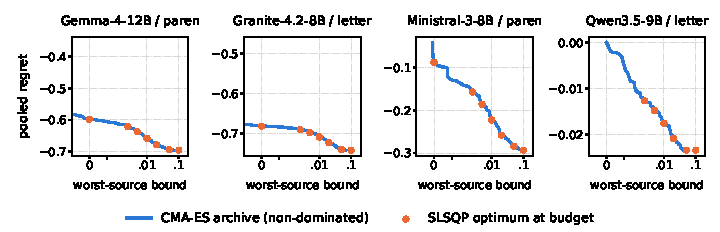
\includegraphics[width=\linewidth]{figures/evo_front.pdf}
\caption{Empirical Pareto fronts of pooled source regret against worst-source bound from all CMA-ES evaluations (line), with the SLSQP optimum for each budget $\varepsilon$ (dots), for four units. The dots lie on the evolutionary front.}
\label{fig:front}
\end{figure}

\paragraph{Evolving the structure helps.}
Where the solver for the weights is already globally adequate, the structure of the field is not: Evo-RB improves on RB-Cal on every roster (Table~\ref{tab:main}).
On LOTO its mean gain is \LotoEvoDelta{} against \LotoRbDelta{} with \LotoEvoHarm{} harmed unit against \LotoRbHarm, which meets the acceptance rule fixed before the run, and its mean ECE drops from \LotoRbEce{} to \LotoEvoEce.
The improvement on the secondary rosters is smaller (0.005--0.010 nats) but has the same sign everywhere.
The cost is computational: 300 inner solves per unit instead of one.

\paragraph{What did not work.}\label{sec:negative}
We report four attempts to close the remaining gap, all evaluated on LOTO (design data) unless stated.
(i) \emph{Dropping the margin} ($z=0$) adds harm without gain (\LotoRelaxDelta, \LotoRelaxHarm{} harmed units).
(ii) \emph{Peer consensus features}, the probability the other four models give to a model's top answer, add little (\LotoPeerDelta, \LotoPeerHarm{} harmed unit).
(iii) \emph{Averaging the two answer orders} before calibration lowers log-loss by \LotoAvgIdRaw{} nats by itself and helps every method; on that averaged base RB-Cal keeps a smaller share of the pooled gain (\LotoAvgRbSame{} vs.\ \LotoAvgPooledSame{} relative to the averaged model), so comparisons must hold the base fixed, as Table~\ref{tab:main} does.
(iv) \emph{A task-level switch} between pooled TS and RB-Cal driven by order and template consistency looked strong on LOTO with thresholds chosen on the other tasks (\SwitchLotoDelta, \SwitchLotoHarm{} harmed units) but failed its pre-registered test on C4 (\SwitchCfourDelta, \SwitchCfourHarm{} harmed units).
An oracle switch would reach \OracleDelta{} on LOTO with no harm; the signals predict where pooled TS harms (AUROC \AucTemplate) but not where it beats RB-Cal (\AucBeats).

\paragraph{Where safety breaks.}
C4 consists of synthetic reasoning tasks far from all sources.
There every method harms units, RB-Cal and Evo-RB seven of 100, the unconstrained methods 13--14; the largest share is on temporal sequences, on which the uncalibrated models are already well calibrated (mean ECE \CfourTempIdEce) and pooled TS harms \CfourTempPooledHarm{} of 10 units.
This is the regime the transfer bound of Section~\ref{sec:method} leaves uncontrolled: a budget on sources says nothing about targets that resemble no mixture of them.

\section{Discussion and Limitations}
The evidence supports a trade-off, not dominance: budgeting every source keeps about \RetainEvo\% of the gain of unconstrained calibration while harming roughly \HarmRatio{} times fewer task units, and an evolution strategy improves the field's structure on top of exact weights.
Several limitations apply.
The method was developed over sequential rounds; only C3 and C4 are out-of-sample for RB-Cal and none of the rosters is for Evo-RB, whose acceptance rests on LOTO, which reuses hyperparameters selected with the held-out task present.
Thermometer-P and ATS-P are probability-feature adaptations and may be weaker than the hidden-state originals.
The order-consistency features double the inference cost.
All tasks are multiple choice with letter probabilities, the models have 7--12B parameters, and the confidence-bound margin is a heuristic, not a simultaneous guarantee.
Safety did not transfer to the far roster C4.
A natural next step for evolutionary computation is a many-objective search over per-unit budgets, which the per-model differences between the Pareto fronts in Fig.~\ref{fig:front} suggest.

\section{Conclusion}
Calibration transfer is a many-objective problem, and its averages hide the tasks it harms.
Solving its $\varepsilon$-constraint scalarisation over a label-free temperature field, certifying the solutions with CMA-ES and evolving the field's structure gives a calibrator that harms \AggEvoHarmRate\% of \NTotal{} target task units, against \AggThermoHarmRate--\AggAtsHarmRate\% for pooled and learned-temperature baselines, at \RetainEvo\% of their mean gain.
Code, per-row probabilities for all models, pre-registrations and the protocol log are provided as anonymised supplementary material.

\bibliographystyle{splncs04}
\bibliography{refs}
\end{document}
